\documentclass[conference]{IEEEtran}
\IEEEoverridecommandlockouts
% The preceding line is only needed to identify funding in the first footnote. If that is unneeded, please comment it out.
\usepackage{cite}
\usepackage{amsmath,amssymb,amsfonts}
\usepackage{algorithmic}
\usepackage{graphicx}
\usepackage{textcomp}
\usepackage{xcolor}
\def\BibTeX{{\rm B\kern-.05em{\sc i\kern-.025em b}\kern-.08em
    T\kern-.1667em\lower.7ex\hbox{E}\kern-.125emX}}
\begin{document}

\title{Learning to detect robots from artificial images\\
%{\footnotesize \textsuperscript{*}Note: Sub-titles are not captured in Xplore and
%should not be used}
\thanks{Identify applicable funding agency here. If none, delete this.}
}

\author{\IEEEauthorblockN{1\textsuperscript{st} Christoph Heindl}
\IEEEauthorblockA{\textit{Visual Computing} \\
\textit{PROFACTOR GmbH}\\
4407 Steyr, Austria \\
christoph.heindl@profactor.at}
\and
\IEEEauthorblockN{2\textsuperscript{nd} Sebastian Zambal}
\IEEEauthorblockA{\textit{Machine Vision} \\
\textit{PROFACTOR GmbH}\\
4407 Steyr, Austria \\
sebastian.zambal@profactor.at}
%%%\and
%%%\IEEEauthorblockN{3\textsuperscript{rd} Markus Ikeda}
%%%\IEEEauthorblockA{\textit{Robotics} \\
%%%\textit{PROFACTOR GmbH}\\
%%%4407 Stey, Austria \\
%%%markus.ikeda@profactor.at}
%%%\and
%%%\IEEEauthorblockN{~~~~~~~~~4\textsuperscript{th} Christian Eitzinger~~~~~~~~~}
%%%\IEEEauthorblockA{\textit{Machine Vision} \\
%%%\textit{PROFACTOR GmbH}\\
%%%4407 Stey, Austria \\
%%%christian.eitzinger@profactor.at}
%%%\and
%%%\IEEEauthorblockN{5\textsuperscript{th} Andreas Pichler}
%%%\IEEEauthorblockA{\textit{Robotics} \\
%%%\textit{PROFACTOR GmbH}\\
%%%4407 Stey, Austria \\
%%%anreas.pichler@profactor.at}
\and
\IEEEauthorblockN{6\textsuperscript{th} Josef Scharinger}
\IEEEauthorblockA{\textit{Institute of Computational Perception} \\
\textit{Johannes Kepler University}\\
4040 Linz \\
josef.scharinger@jku.at}
}

\maketitle

\begin{abstract}
Impressive results have been achieved in computer vision via machine learning methods over the last years. However, for many highly specialized industrial applications these methods cannot directly be applied due to the lack of large amounts of training data. In this paper we propose a software framework that provides artificial data. Such artificial data opens the door for machine learning even when it is hard or impossible to acquire real data. The presented system is flexible in the sense that it supports image data generation in a flexible way. We show how artificial images can directly be used in pytorch to perform deep neural network training. 
\end{abstract}

\begin{IEEEkeywords}
machine learning, artificial data, data augmentation
\end{IEEEkeywords}

\section{Introduction}
The impressive results of supervised deep learning in the field of robotics and computer vision are to large extent due to the availability of annotated data sets. Up until recently most of the annotation was carried out by domain experts. This time consuming process significantly slows down the progress of deep learning efforts. In many tasks it is difficult, in most niche areas impossible, to obtain strong supervision because of the high costs.

Exposed to this bottleneck, new fields of research have opened up. Active learning \cite{druck2009active, settles2012active, cakmak2012designing} attempts to use human experts in a more targeted way by focusing on samples that seem to of highest value for learning task. Semi-supervised learning \cite{chapelle2009semi, salimans2016improved, zhu2006semi} combines large unlabeled data sets with smaller labeled data sets through structural assumptions, such as smoothness or low-dimensionality constraints. Transfer learning \cite{pratt1993discriminability, ventura2007theoretical, pan2010survey} exploits the fact that models trained on specific tasks can be adapted to related problems using fewer training samples. Weak supervision \cite{ratner2016data, zhou2017brief} is motivated by leveraging less precise, higher level supervision that is often easier to obtain. This includes heuristics, weak or biased classifiers, unreliable non-experts. 

% https://hazyresearch.github.io/snorkel/blog/ws_blog_post.html

In contrast to the methods mentioned above, synthetic data generation drops the necessity for real world annotated data in favor of artificial data sources. Synthesized data is available in virtually infinite variety and is de-facto auto-labelled. This has led to variety of successful applications in different domains: Jaderberg et al. \cite{jaderberg2014synthetic} have demonstrated natural scene text recognition from synthetic data, Peng et al. \cite{peng2015learning} trained object detectors from 3d models and Johnson et al. \cite{2017_Johnson_DrivingInTheMatrix} used photo-realistic computer rendering captured from a game engine to train car detectors. 

A common theme to all of these synthetic approaches is the following: (a) a simulator engine generators artificial training data, (b) the generated data is stored to disk and (c) the offline data stack is used for training. The shortcomings to this procedure are early training data commitment and the lack of adaptability of data generation to training demands.

In this paper we propose a principled way of generating artificial training data from a 3D simulator engine that is directly looped into the training procedure, thereby avoiding early data commitment. A bi-directional communication channel enables the training procedure to request random samples with varying priority. We demonstrate the usefulness of our approach to the detection of robot poses in color images using non-realistic computer images.



% idea: bi-directional communication: generate more samples around poses of high error (i.e training procedure communicates back to simulator).






\begin{figure}[htbp]
\centerline{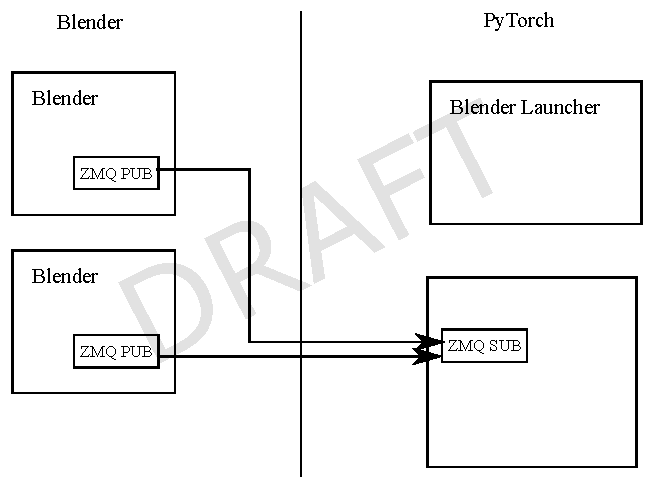
\includegraphics[width=\columnwidth]{figures/architecture/architecture.pdf}}
\caption{\label{fig:architecture} Architecture of our system: Individual instances generate artificially rendered images (left). These are consumed in a pytorch environment for training of deep neural networks (right).}
\label{fig}
\end{figure}


\begin{figure}[htbp]
\centerline{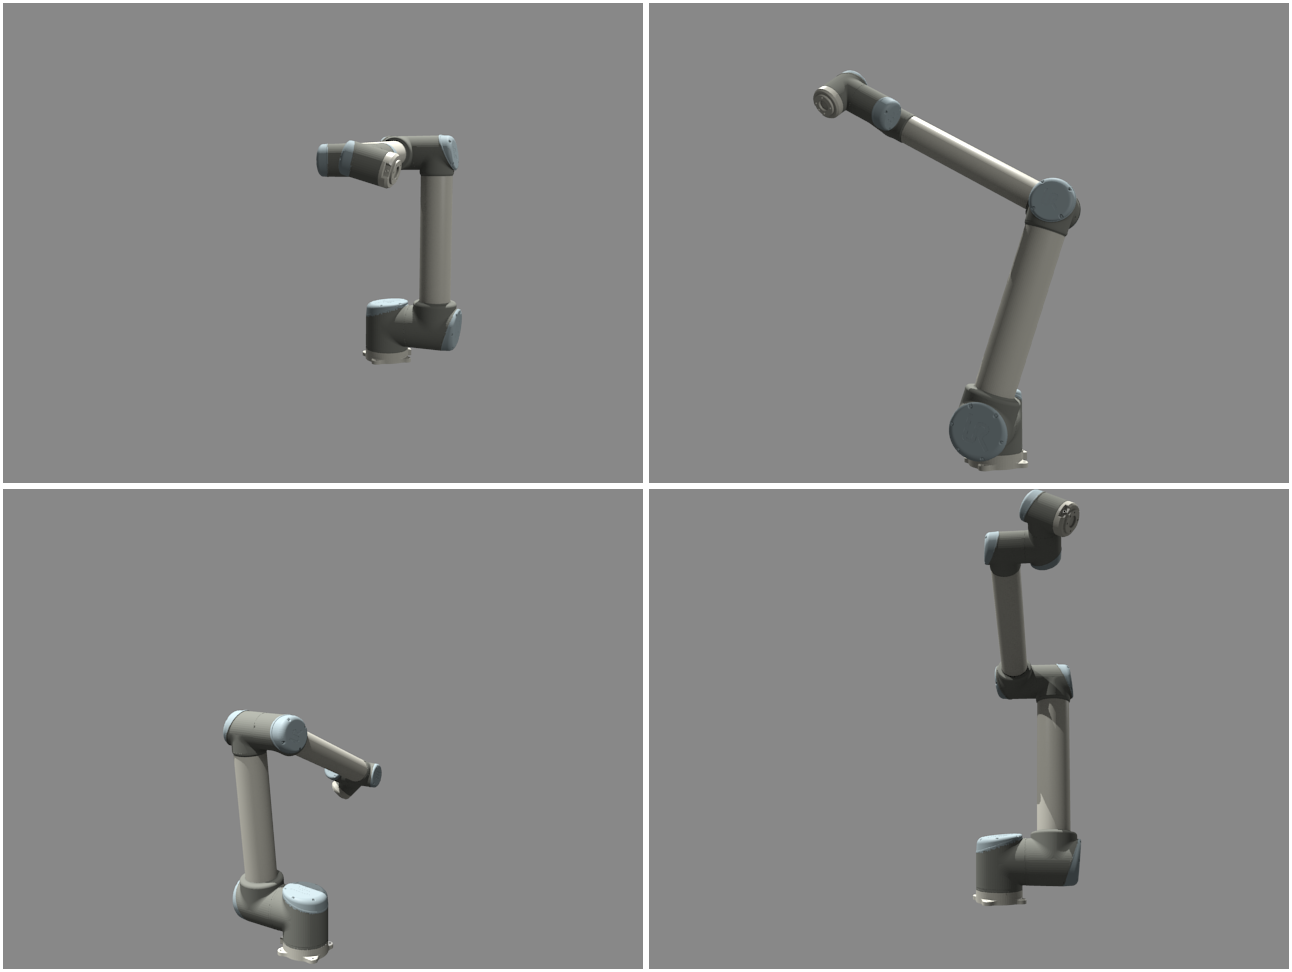
\includegraphics[width=\columnwidth]{figures/examplesUR10/renderedImages.png}}
\caption{\label{fig:architecture} Architecture of our system: Individual instances generate artificially rendered images (left). These are consumed in a pytorch environment for training of deep neural networks (right).}
\label{fig}
\end{figure}


\section{Method}

\subsection{Artificial data and data loaders}

TODO: Outline Python-support of Blender, Explain scripting in Blender, creation of meta-data (joint locations, etc.)...
TODO: Explain basic concepts of PyTorch and DataLoaders, etc.
TODO: Explain ZMQ pipeline, publish/subscribe

\subsection{Joint localization}

TODO: Neural network architecture, network input/output, etc.

\section{Results}

Evaluation UR10, comparison with Staubli
TODO

\begin{table}[htbp]
\caption{Performance evaluation}
\begin{center}
\begin{tabular}{|c|c|}
\hline
\textbf{Blender instance} & \textbf{Runtime ms/batch} \\
\hline
1 & 103 ms ± 5.17 ms \\
\hline
2 & 43.7 ms ± 10.3 ms \\
\hline
\end{tabular}
\label{tab1}
\end{center}
\end{table}

\section*{Acknowledgment}

Work presented in this paper has received funding from the European Union’s Horizon 2020 research and innovation programme under grant agreement No 721362 (project “ZAero”).

\small
\bibliographystyle{ieeetr}
\bibliography{biblio}



%%%\begin{thebibliography}{00}
%%%\bibitem{b1} G. Eason, B. Noble, and I. N. Sneddon, ``On certain integrals of Lipschitz-Hankel type involving products of Bessel functions,'' Phil. Trans. Roy. Soc. London, vol. A247, pp. 529--551, April 1955.
%%%\bibitem{b2} J. Clerk Maxwell, A Treatise on Electricity and Magnetism, 3rd ed., vol. 2. Oxford: Clarendon, 1892, pp.68--73.
%%%\bibitem{b3} I. S. Jacobs and C. P. Bean, ``Fine particles, thin films and exchange anisotropy,'' in Magnetism, vol. III, G. T. Rado and H. Suhl, Eds. New York: Academic, 1963, pp. 271--350.
%%%\bibitem{b4} K. Elissa, ``Title of paper if known,'' unpublished.
%%%\bibitem{b5} R. Nicole, ``Title of paper with only first word capitalized,'' J. Name Stand. Abbrev., in press.
%%%\bibitem{b6} Y. Yorozu, M. Hirano, K. Oka, and Y. Tagawa, ``Electron spectroscopy studies on magneto-optical media and plastic substrate interface,'' IEEE Transl. J. Magn. Japan, vol. 2, pp. 740--741, August 1987 [Digests 9th Annual Conf. Magnetics Japan, p. 301, 1982].
%%%\bibitem{b7} M. Young, The Technical Writer's Handbook. Mill Valley, CA: University Science, 1989.
%%%\end{thebibliography}
%%%\vspace{12pt}
%%%\color{red}
%%%IEEE conference templates contain guidance text for composing and formatting conference papers. Please ensure that all template text is removed from your conference paper prior to submission to the conference. Failure to remove the template text from your paper may result in your paper not being published.

\end{document}
